\documentclass[12pt, a4paper, oneside]{ctexart}
\usepackage{amsmath, amsthm, amssymb, bm, graphicx, hyperref, mathrsfs, xcolor}
\usepackage{pgfplots, tikz, tikz-qtree, listings, framed}
\usepackage{geometry}
\geometry{left=1.2cm,right=1.2cm,top=1.4cm,bottom=1.2cm}

\title{\textbf{《程序设计基础》大作业\\ ——通讯录管理程序}}
\author{Shiyuu}
\date{\today}
\linespread{1.1}
%定义了题目,解答,注记三个环境
\definecolor{shadecolor}{RGB}{222, 227, 230}
\newcounter{problemname}
\newenvironment{problem}{\stepcounter{problemname}\par\noindent\textbf{题目}}{\\\par}
\newenvironment{solution}{\par\noindent\textbf{解答. }}{\\\par}
\newenvironment{problem*}
    {\begin{shaded}\par\noindent}{\end{shaded}\par}
\newenvironment{note}{\par\noindent\large{\textbf{题目\arabic{problemname}的注记. }}}{\\\par}

\definecolor{mygreen}{rgb}{0,0.6,0}
\definecolor{mygray}{rgb}{0.5,0.5,0.5}
\definecolor{mymauve}{rgb}{0.58,0,0.82}

%cpp代码环境设置

\lstset{%
	language=C++,
	backgroundcolor=\color{white},
	basicstyle=\tiny,
	breakatwhitespace=false,
	breaklines=true,
	captionpos=t,
    frame=shadowbox,
    rulesepcolor= \color{red!20!green!20!blue!20},
	commentstyle=\color{mygreen},
	deletekeywords={...},
	escapeinside={\%*}{*)},
	extendedchars=true,
	frame=single,
	keepspaces=true,
	keywordstyle=\color{blue},
	language=Octave,
	%otherkeywords={*,...},
	numbers=left,
	numbersep=5pt,
	numberstyle=\tiny\color{mygray},
	rulecolor=\color{black},
	showspaces=false,
	showstringspaces=false,
	showtabs=false,
	stepnumber=1,
	stringstyle=\color{mymauve},
	tabsize=4,
	title=\lstname
}
\lstdefinestyle{customcpp}{
	belowcaptionskip=0pt,
	breaklines=true,
	%frame=L,
	xleftmargin=\parindent,
	language=C++,
	showstringspaces=false,
	basicstyle=\scriptsize\ttfamily,
	keywordstyle=\bfseries\color{green!40!black},
	commentstyle=\itshape\color{purple!40!black},
	identifierstyle=\color{blue},
	stringstyle=\color{orange},
}
\lstset{escapechar=@,style=customcpp}

%----------------------------------
\begin{document}
\maketitle

\section{项目分析}
\subsection{问题描述}
\begin{problem*}
    \\ \textbf{通讯录管理系统} \\
    问题描述及设计要求:\\
    设计一个通讯录管理系统,要求实现以下功能:\\
    (1) 添加联系人信息(包括电话号码、姓名、工作单位和住址),并可连续添加;\\
    (2) 查找联系人信息(按电话号码查找,返回联系人的所有信息);\\
    (3) 删除联系人信息;\\
    (4) 修改联系人信息;\\
    (5) 对联系人信息按姓名首字母进行排序(升序);\\
    (6) 统计联系人个数;\\
    (7) 显示所有联系人信息;\\
    (8) 退出系统。\\ \\
    附加功能:\\
    (1) 清空通讯录;\\
    (2) 检查输入的合法性(如电话号码必须为11位纯数字,不得出现字母、标点或中文);\\
    (3) 在指定联系人信息记录后面插入新记录;\\
    (4) 以外部文件读写的方式保存通讯录。
\end{problem*}
\subsection{问题分析}
这是一个典型的数据管理型的程序。注意到题目要求的添加、查找、删除、修改等要求,考虑使用二叉树数据结构存储通讯录信息。为了保证二叉搜索树在数据量很大时的效率,考虑使用AVL二叉树数据结构。同时,题目要求我们将通讯录数据保存到外部文件中,所以还要编写相应的文件读写程序。为了程序的运行稳定性和可移植性,需要编写动态存储的程序。最后为了方便管理和修改功能,把项目中关于二叉树数据类型抽象为一个接口,封装到单独的文件中,也就是创建抽象数据类型(ADT),而管理交互界面(GUI)的主文件则单独列出,编译时进行多文件编译。

通过这次大作业,可以:
\begin{enumerate}
    \item 掌握AVL二叉树的创建与操作
    \item 掌握抽象数据结构(ADT)的创建与使用
    \item 掌握多文件项目的基本方法
    \item 进一步体会结构体的使用方法
    \item 练习文件读写操作
\end{enumerate}

\subsection{基本知识}
\subsubsection{AVL二叉树}
AVL树是一种自平衡二叉搜索树,最早由俄国数学家Adel'son-Vel'skii和Landis发明。它通过在树的结构体中植入一个高度因子,计算每个节点的左子树和右子树高度之差,通过左旋和右旋操作使这个差值不超过1。

AVL树的每个节点都存储了一个键值,并且满足以下性质:

\begin{itemize}
    \item 左子树和右子树的高度差不超过1。
    \item 对于每个节点,其左子树中的所有键值都小于该节点的键值,右子树中的所有键值都大于该节点的键值。
    \item 每个子树都是AVL树。
    \item AVL树的插入和删除操作都会涉及到旋转操作,旋转操作分为左旋和右旋。左旋和右旋都是以某个节点为支点,将该节点和其子树进行旋转,以达到平衡的目的。
\end{itemize}

AVL树的自平衡基于两个基本操作,由于树中节点排列顺序一定,所以可以通过修改父级节点中的指针来完成节点高度的提升和降低,这两个操作称为左旋(L-Rotation)和右旋(R-Rotation)。考虑以下插入操作,其中M表示高度大于2的子树,阿拉伯数字表示空指针:

\noindent
\begin{minipage}{0.49\linewidth}
\begin{framed}
    \begin{center}
        \textbf{R-Rotation}
    \end{center}
    \begin{tikzpicture}[grow=down]{line width=0.45}
        \centering
        \Tree
        [.A 
        [.B [.D [.$M_1$ ] [.$M_2$ ] ] [.1 ] ] 
        [.C [.2 ] [.3 ]]
        ]
    \end{tikzpicture}
    %
    $\stackrel{\text{右旋}}{\Longrightarrow}$
    \begin{tikzpicture}[grow=down]{line width=0.45}
        \centering
        \Tree
        [.B 
        [.D [.$M_1$ ] [.$M_2$ ] ] [.A [.1 ] [.C [.2 ] [.3 ]]]
        ]
    \end{tikzpicture}
\end{framed}
\end{minipage}
%
\begin{minipage}{0.49\linewidth}
\begin{framed}
    \begin{center}
        \textbf{L-Rotation}
    \end{center}
    \begin{tikzpicture}[grow'=down]{line width=0.45}
        \centering
        \Tree
        [.A 
        [.C [.D [.$M_1$ ] [.$M_2$ ] ] [.1 ] ] 
        [.B [.2 ] [.3 ]]
        ]
    \end{tikzpicture}
    %
    $\stackrel{\text{左旋}}{\Longrightarrow}$
    \begin{tikzpicture}[grow'=down]{line width=0.45}
        \centering
        \Tree
        [.C 
        [.D [.$M_1$ ] [.$M_2$ ] ] [.A [.1 ] [.B [.2 ] [.3 ]]]
        ]
    \end{tikzpicture}
\end{framed}
\end{minipage}

在这两个对称的操作中,以右旋为例,检测到B的高度差绝对值大于1,于是将B节点提拔为根节点,其右节点指向它的父节点A,A的左指针则指向B原先的右指针指向的地址。这样一来就实现了树的平衡。

而对于M接在“中间”位置上的时候,情况则变得麻烦一点,但我们不难看出这时的平衡可以通过两次左右旋的交替来完成,这时子树在$M_1$或是在$M_2$上是等价的:

\noindent
\begin{center}
\begin{minipage}{0.85\linewidth}
\begin{framed}
    \begin{center}
        \textbf{LR-Rotation}
    \end{center}
    \begin{tikzpicture}[grow=down]{line width=0.45}
        \centering
        \Tree
        [
        .A 
        [.B [.1 ] [.D [.$M_1$ ] [.$M_2$ ]]] [.C [.2 ] [.3 ]]
        ]
    \end{tikzpicture}
    %
    \quad$\stackrel{\text{左旋}}{\Longrightarrow}$\quad
    \begin{tikzpicture}[grow=down]{line width=0.45}
        \centering
        \Tree
        [
        .A 
        [.D [.B [.1 ] [.$M_1$ ]] [.$M_2$ ]] 
        [.C [.2 ] [.3 ]]
        ]
    \end{tikzpicture}
    %
    \quad$\stackrel{\text{右旋}}{\Longrightarrow}$\quad
    \begin{tikzpicture}[grow=down]{line width=0.45}
        \centering
        \Tree
        [
        .D 
        [.B [.1 ] [.$M_1$ ]] [.A [.$M_2$ ] [.C [.2 ] [.3 ]]]
        ]
    \end{tikzpicture}
\end{framed}
\end{minipage}
\end{center}

观察到先绕B进行左旋,再绕A进行了右旋,最终把2提拔为根节点,使$M_1$、$M_1$\noindent 落在等价高度上,树恢复了平衡。注意在两个操作中,围绕的节点的子节点都是2。同理:

\noindent
\begin{center}
\begin{minipage}{0.85\linewidth}
\begin{framed}
    \begin{center}
        \textbf{RL-Rotation}
    \end{center}
    \begin{tikzpicture}[grow'=down]{line width=0.45}
        \centering
        \Tree
        [
        .A 
        [.C [.3 ] [.D [.$M_2$ ] [.$M_1$ ]]] [.B [.2 ] [.1 ]]
        ]
    \end{tikzpicture}
    %
    \quad$\stackrel{\text{右旋}}{\Longrightarrow}$\quad
    \begin{tikzpicture}[grow'=down]{line width=0.45}
        \centering
        \Tree
        [
        .A 
        [.D [.C [.3 ] [.$M_2$ ]] [.$M_1$ ]] 
        [.B [.2 ] [.1 ]]
        ]
    \end{tikzpicture}
    %
    \quad$\stackrel{\text{左旋}}{\Longrightarrow}$\quad
    \begin{tikzpicture}[grow'=down]{line width=0.45}
        \centering
        \Tree
        [
        .D 
        [.C [.3 ] [.$M_2$ ]] [.A [.$M_1$ ] [.B [.2 ] [.1 ]]]
        ]
    \end{tikzpicture}
\end{framed}
\end{minipage}
\end{center}

\indent AVL树的查找操作和二叉搜索树一样,时间复杂度为o(log n)。由于AVL树的平衡性质,它的插入、删除、查找等操作都具有较稳定的时间复杂度。但是AVL树对于频繁的插入和删除操作,会频繁地进行旋转操作,导致效率下降,因此在这种情况下,可以使用其他自平衡树,如红黑树。

\subsubsection{抽象数据类型}
抽象数据类型(ADT)是一种数据类型的数学模型,其定义仅依赖于它的行为和特征,而不依赖于其具体的实现。它描述了一组数据和定义在这组数据上的一组操作,这些操作可以被认为是一个黑盒子,其内部的实现细节被隐藏。ADT 不考虑具体的实现方式,只关注数据的抽象行为和操作。

一个抽象数据类型通常包含三个方面:

\begin{enumerate}
    \item 数据表示:定义 ADT 中的数据结构,通常用类或结构体来实现。
    \item 数据操作:定义一组在数据结构上的操作,比如增加、删除、查找、修改等。
    \item 约束条件:对数据的操作进行限制,以确保数据结构的正确性。
\end{enumerate}

使用抽象数据类型可以帮助我们将程序设计的重点放在程序的功能实现上,而不用关注具体的实现方式。这也使得代码的维护和扩展变得更加容易,因为我们只需要关注 ADT 的定义和使用方法,而不用关心其具体实现细节。

比如,在本项目中,可以使用AVL树的抽象数据类型,在一个头文件AVLTree.h中定义AVL树的结构类型和操作函数原型,在AVLTree.c文件中编写树操作的函数,并通过static关键字将一些函数的作用域限定在一个文件内。还可以通过编写Format.h文件来定义通讯录数据类型,便于修改;编写gui.c文件提供给主文件调用的交互界面。

\section{代码编写}
\subsection{定义类型}
首先需要定义元素的类型:在本例中包括姓名、电话号码、住址、工作单位。然后是二叉节点的类型:每一个节点包含一个元素(Item类型)和两个指向下级节点的指针,然后定义一个树结构(Tree)包含指向根节点的指针和树中元素的个数。还需要定义查找时使用的父子节点结构,定义为Pair结构,包含指向父节点和子节点的指针。
\begin{framed}
\begin{lstlisting}[language=C++]
    AVLTree.h -AVL树ADT原型

    //二叉树节点结构体
    typedef struct trnode
    {
        Item item;
        int height;
        struct trnode * left;
        struct trnode * right;
    } Trnode;

    //二叉树访问结构体
    typedef struct tree
    {
        Trnode * root;
        int size;
    } Tree;

    //二叉查找结构体
    typedef struct pair
    {
        Trnode * parent;
        Trnode * child;
    } Pair;
\end{lstlisting}
\end{framed}
\begin{framed}
\begin{lstlisting}[language=C++]
    //Format.h -电话簿信息结构定义
    typedef struct item
    {
        char name[MAXLINE];
        char phone[PHONENUMBERLINE];
        char workplace[MAXLINE];
        char address[MAXLINE];
    } Item;
\end{lstlisting}
\end{framed}

\subsection{建立接口}
在编写程序之前,先将ADT接口将要实现的功能抽象地写在一个头文件中,并提供函数原型。
\begin{framed}
\begin{lstlisting}[language=C++]
    //AVLTree.h -AVL树ADT原型
    //树中不允许重复数据
    //左子树的所有项都在根节点的前面,右子树的所有项都在根节点的后面
    
    /*函数原型*/

    //O:将树初始化为空
    //P:NULL
    //E:树被初始化为空,并返回一个指向Tree的指针
    Tree * InitializeTree(void);

    //O:确定树是否为空
    //P:ptree指向一个Tree类型
    //E:若为空,返回true,否则返回false
    bool IsTreeEmpty(const Tree * ptree);

    //O:确定树是否已满
    //P:ptree指向一个Tree类型
    //E:若为空,返回true,否则返回false
    bool IsTreeFull(const Tree * ptree);

    //O:确定树中的项数
    //P:ptree指向一个Tree类型
    //E:返回一个树的项数
    int TreeItemCount(const Tree * ptree);

    //O:在树中添加一个项
    //P:pi指向待添加项的地址,ptree指向要添加到的树
    //E:如果可以添加,则返回该节点及其父级
    bool AddItem(const Item * pi, Tree * ptree);

    //O:在树中删除一个项
    //P:pi指向待删除项的地址,ptree指向要操作的树
    //E:如果可以删除,则返回true,同时将该项从树中删除,否则返回false
    bool DelItem(const Item * pi, Tree * ptree);

    //O:在树中查找一个项
    //P:pi指向待查找项的地址,ptree指向要操作的树
    //E:如果查找到,则返回true,否则返回false
    bool InTree(const Item * pi, const Tree * ptree);

    //O:清空树
    //P:ptree指向一个Tree类型
    //E:ptree指向的Tree被清空
    void DelAll(Tree * ptree);

    //O:将通讯录写入指定文件流
    //P:ptree指向一个Tree类型,File指向一个文件
    //E:ptree指向的Tree中的每一个Item以指定顺序写入文件流
    bool TreeWritef(const Tree * ptree, FILE * fp, const char * order);

    //O:从指定文件流中读取一个树
    //P:ptree指向一个Tree类型,File指向一个文件
    //E:ptree指向的Tree中的每一个Item以指定顺序写入文件流并自平衡
    bool TreeReadf(Tree * ptree, FILE * fp);

    //O:在交互页面(标准输入流中)读取树的一个元素
    //P:ptree指向一个Tree类型
    //E:ptree指向的树中的Item写入文件流并自平衡
    bool TreeReadOne(Tree * ptree);

    //O:在输入流中显示二叉树结构
    //P:ptree指向一个Tree类型,fp是一个文件指针
    //E:ptree指向的树以图表方式显示在fp指向的文件流中,以name为标签
    bool ShowTree(Tree *ptree, FILE * fp);

    //O:在指定文件流中输出一个Item结构
    //P:fp是一个文件指针
    //E:在fp指向的文件中格式化打印了一个item中的数据
    bool PrintItem(const Item item, FILE * fp);

    //O:在树中搜索节点
    //P:pi指向一个Item结构,ptree指向一个Tree结构
    //O:值为pi指向的值的节点,返回以这个节点为子节点的Pair结构
    Pair SeekItem(const Item * pi, const Tree * ptree);
\end{lstlisting}
\end{framed}
\subsection{实现接口}
    然后单独在AVLTree.c文件中编写树操作的函数。有一些函数是比较基本的二叉树函数,比如中序遍历、递归显示元素、判断树是否为空、删除树等,这里不全部详细展开,只来看几个比较重要的函数。
\begin{framed}
\begin{lstlisting}[language=C++]
    bool InTree(const Item * pi, const Tree * ptree)
    {
        return (SeekItem(pi, ptree).child == NULL) ? false : true;
    }
    //节点导航
    static bool ToLeft(const Item * i1, const Item * i2)
    {
        int comp1;
        if((comp1 = strcmp(i1->name, i2->name)) < 0)
            return true;
        else
            return false;
    }

    static bool ToRight(const Item * i1, const Item * i2)
    {
        int comp1;
        if((comp1 = strcmp(i1->name, i2->name)) > 0)
            return true;
        else
            return false;
    }

    //搜索节点(递归方法)
    Pair SeekItem(const Item * pi, const Tree * ptree)
    {
        Pair look;
        look.parent = NULL;
        look.child = ptree->root;
        if(look.child == NULL)
            return look;
        else
            return RecuSeek(pi, look);
    }

    static Pair RecuSeek(const Item * pi, Pair look)
    {
        if(look.child == NULL)
            return look;
        else if(ToLeft(pi, &(look.child->item)))
        {
            look.parent = look.child;
            look.child = look.child->left;
            return RecuSeek(pi, look);
        }
        else if(ToRight(pi, &(look.child->item)))
        {
            look.parent = look.child;
            look.child = look.child->right;
            return RecuSeek(pi, look);
        }
        else 
            return look;
    }
\end{lstlisting}
\end{framed}
这里主要的函数是Intree(),但它本身只有一行代码,而把工作交给了调用的代码来完成操作。而调用的SeekItem()和ToLeft()等函数声明时均带上了static关键字,这是为了将函数作用域限制在AVLTree.c内部,只向外界展示Intree()函数,避免误调用。

\begin{framed}
\begin{lstlisting}[language=C++]
    static Trnode * AddNode(Trnode * new_node, Trnode * root)
    {   
        Pair current;
        current.parent = root;
        new_node->height = root->height + 1;  
        if(ToLeft(&new_node->item, &root->item))
        {  
            if(root->left == NULL)
            {
                root->left = new_node;
                current.child = root->left;
            }
            else
            {
                current.child = AddNode(new_node, root->left);//递归查找子树
                current.parent->left = current.child;
            }
        }
        else if(ToRight(&new_node->item, &root->item))
        {
            if(root->right == NULL)
            {
                root->right = new_node;
                current.child = root->right;
            }
            else
            {
                current.child = AddNode(new_node, root->right);//递归查找子树
                current.parent->right = current.child;
            }
        }
        else
        {
            fprintf(stderr, "FAIL TO ADD A NODE");
            exit(EXIT_FAILURE);
        }
        //添加完成后检测父节点高度因子,从下到上逐次旋转
        //高度因子为左最长子树高度-右,若为正数则R或LR,若为负数则L或RL
        return Rotation(current);
    }
    
    //执行旋转操作,返回新的根节点
    static Trnode * Rotation(Pair current)
    {
        int Rotate = GetHeightFactor(current.parent);
        if(Rotate > 1)
        {   
            if(GetHeightFactor(current.child) < 0)
                current.parent->left = LeftRotate(current.child);
            return RightRotate(current.parent);
        }
        else if(Rotate < -1)
        {   
            if(GetHeightFactor(current.child) > 0)
                current.parent->right = RightRotate(current.child);
            return LeftRotate(current.parent);
        }
        else
            return current.parent;
    }
    
    static int GetHeight(const Trnode * root)
    {   
        if(root == NULL)
            return 0;
        if(root->left == NULL && root->right == NULL)
            return root->height;
        else if(root->left == NULL && root->right != NULL)
            return GetHeight(root->right);
        else if(root->left != NULL && root->right == NULL)
            return GetHeight(root->left);
        else
            return MAX(GetHeight(root->left), GetHeight(root->right));
    }
    
    static int GetHeightFactor(const Trnode * root)
    {   
        if(root == NULL)
            return 0;
        else if(root->left == NULL && root->right != NULL)
            return root->height - GetHeight(root->right);
        else if(root->left != NULL && root->right == NULL)
            return GetHeight(root->left) - root->height;
        else
            return GetHeight(root->left) - GetHeight(root->right);
    }
    
    static void ChangeHeight(Trnode * root, int val)
    {
        if(root != NULL)
        {
            ChangeHeight(root->left, val);
            root->height += val;
            ChangeHeight(root->right, val);
        }
    }
    
    static Trnode * RightRotate(Trnode * root)
    {   
        Trnode * new_root = NULL;
        new_root = root->left;
        //左子树高度全部减1,右子树和根节点高度全部加1
        ChangeHeight(root->left, -1);
        root->height += 1;
        ChangeHeight(root->right, 1);
        //移动指针
        root->left = (new_root->right == NULL) ? NULL : new_root->right;
        new_root->right = root;
        return new_root;
    }
    
    static Trnode * LeftRotate(Trnode * root)
    {   
        Trnode * new_root = NULL;
        new_root = root->right;
        //右子树高度全部减1,左子树和根节点高度全部加1
        ChangeHeight(root->right, -1);
        root->height += 1;
        ChangeHeight(root->left, 1);
        //移动指针
        root->right = (new_root->left == NULL) ? NULL : new_root->left;
        new_root->left = root;
        return new_root;
    }
\end{lstlisting}
\end{framed}
以上是AVL树插入节点并通过旋转实现自平衡的代码。程序先将新节点插入到应有位置,然后逐层递归获得节点高度因子。若高度因子绝对值大于一,则调用局部函数Rotation()进行旋转,Rotaton()函数基于搜索到的Pair结构对节点、选择调用LeftRotate()和RightRotate()进行旋转。需要注意:如果要执行双旋,则需要对三层节点进行操作。所以LeftRotate()和RightRotate()应该是Pair,用以在递归时传递节点信息。

\begin{framed}
\begin{lstlisting}[language=C++]
    bool TreeWritef(const Tree * ptree, FILE * fp, const char * order)
    {
        if(ptree == NULL)
        {
            return false;
            fprintf(stderr, "TREE DOES NOT EXISTS");
        }
        if(strcmp(order, "DESC"))
            return PrintDESC(ptree->root, fp);
        if(strcmp(order, "ASC"))
            return PrintASC(ptree->root, fp);
        return false;
    }
    
    static bool PrintASC(const Trnode * root, FILE * fp)
    {   
        if(root != NULL)
        {
            PrintASC(root->right, fp);
            fprintf(fp, "Item:\n");
            PrintItem(root->item, fp);
            PrintASC(root->left, fp);
        }
    }
    
    static bool PrintDESC(const Trnode * root, FILE * fp)
    {   
        if(root != NULL)
        {
            PrintDESC(root->left, fp);
            fprintf(fp, "Item:\n");
            PrintItem(root->item, fp);
            PrintDESC(root->right, fp);
        }
    }

    bool TreeReadf(Tree * ptree, FILE * fp) 
    {
        char line[MAXLINE + 50] = {'\0'};//这里挺容易溢出的
        Item item;
        int count = 0;
        while (fgets(line, sizeof(line), fp) != NULL) 
        {   // 逐行读取文件内容
            int i = 0;
            while(line[i] == ' ' || line[i] == '\n' || line[i] == '\t')
                    ++i;//跳过空白符
            if (line[i] == 'N' && line[i + 1] != 'o')
                sscanf(line + i, "NAME: %s", item.name); 
            else if (line[i] == 'P') 
                sscanf(line + i, "PHONE: %s", item.phone); 
            else if (line[i] == 'W')
                sscanf(line + i, "WORKPLACE: %s", item.workplace);
            else if (line[i] == 'A')
            {
                sscanf(line + i, " ADDRESS: %s", item.address); 
                if(!AddItem(&item, ptree))
                    return false;
                ++count;
            }
            else
                continue;
        }
        fprintf(stdout, "Success to read %d piece(s) from "DATABASE"\n", count);
        return true;
    }
    
    bool TreeReadOne(Tree * ptree)
    {
        if(ptree == NULL)
        {
            return false;
            fprintf(stderr, "TREE DOES NOT EXISTS");
        }
        Item * pi = (Item *) malloc(sizeof(Item));
        fputs("Enter the item data.\"RE_\" to restart.\n", stdout);
        const char *filed[] = {"EMPTY", "name", "phone", "workplace", "address"};
        int i = 1;
        for(i = 1; i <= 4; ++i)
        {
            fprintf(stdout, "%s:", *(filed+i));        
            char temp[MAXLINE] = {'\0'};
            fscanf(stdin, "%s", temp);
            if(strcmp(temp, "RE_") == 0)
            {
                i = 0;
                continue;
            }
            if(i == 1)
                strcpy(pi->name, temp);
            if(i == 2)
                strcpy(pi->phone, temp);
            if(i == 3)
                strcpy(pi->workplace, temp);
            if(i == 4)
                strcpy(pi->address, temp);
        }
        int wrong = Islegal(pi);
        if(wrong > 0)
        {
            fprintf(stdout, "ILLEGAL INPUT OF _%s_ TRY AGAIN\n\n", filed[wrong]);
            TreeReadOne(ptree);
        }
        else if(!AddItem(pi, ptree))
        {
            fprintf(stderr, "FAIL TO INSERT\n");
            free(pi);
            return false;
        }
        free(pi);
        fprintf(stdout,"\nDone!\n");
        return true;
    }
    
    //检测输入是否合法,若有错误则返回错误项标号,否则返回0
    static int Islegal(Item * pi)
    {
        if(strlen(pi->phone) != 11)
            return 2;
        for(int i = 0; i < 11; ++i)
            if((pi->phone)[i] < '0' || (pi->phone)[i] > '9')
                return 2;
        return 0;
        //目前只要求检测电话号码的合法性
    }
\end{lstlisting}
\end{framed}
题目要求需要从文件中读取并将记录写入文件,所以编写了bool TreeWritef()函数向指定文件流中写入联系人数据,并添加了可递增和递减显示的选项。这个函数向stdout写入时即可在屏幕终端显示。TreeReadf()则用于从文件流中批量读取联系人信息;TreeReadOne()则是从标准输入流中一次读取一个联系人的信息。

\subsection{交互界面}
最后在另外一个文件中调用显示页面函数ShowGUI(),并在main()中建立一个循环,以多次操作。
\begin{framed}
\begin{lstlisting}[language=C++]
    //TelephoneBook.c -程序主函数&图形化界面
    #include <stdio.h>
    #include <stdlib.h>
    #include <ctype.h>
    #include <string.h>
    #include <stdbool.h>
    #include "AVLTree.h"
    #include "Format.h"
    //#define DATABASE diyname
    
    int main(void)//日后可加启动参数
    {
        printf("Initializing GUI.....Done!\n");
    
        FILE * fpr = fopen(DATABASE, "r");
        FILE * fpw = NULL;
        Tree * ptree = InitializeTree();
        char line[MAXLINE] = {'\0'};
        if(!TreeReadf(ptree, fpr))
        {
            fprintf(stderr, "FAIL TO READ FROM FILE\n");
            exit(EXIT_FAILURE);
        }
        int choice = 7;
        while(true)
        {   
            printf("\n\nPress Enter....");
            getchar();
            choice = ShowGUI();
            if(choice == 0)
            {
                fprintf(stderr, "FAIL TO SHOW GUI\n");
                exit(EXIT_FAILURE);
            }
            switch (choice)
            {
            case 1:
                if(!ShowAllContacts(ptree))
                    printf("FAIL TO SHOW ALL CONTACTS");
                break;
            case 2:
                printf("\nEnter the contact's phone to search: ");
                scanf("%s", line);getchar();
                if(IsContact(ptree->root, line, stdout) == 0)
                    printf("\nNo data found.\n");
                break;
            case 3:
                printf("\nEnter the contact's name to search: ");
                scanf("%s", line);getchar();
                UpdateContact(ptree, line);
                break;
            case 4:
                printf("\nStart adding :\n");
                char ch = 'Y';
                while(true)
                {
                    TreeReadOne(ptree);
                    printf("\nContinue to add? (Y/N) :");
                    getchar();scanf("%c", &ch);getchar();
                    if(ch == 'Y')
                        continue;
                    else
                        break;
                }
                break;
            case 5:
                printf("\nEnter the contact's name to delete: ");
                scanf("%s", line);getchar();
                Item item;
                strcpy(item.name, line);
                Trnode *node;
                node = SeekItem(&item, ptree).child;
                if(node == NULL)
                {
                    printf("\nFind no data.\n");
                    break;
                }
                else
                    DelItem(&(node->item), ptree);
                printf("\nDeleted.\n");
                break;
            case 6:
                printf("\nCurrent number in phone book : %d \n", TreeItemCount(ptree));
                break;
            case 7:
                fpw = fopen(DATABASE, "w");//清空文件
                DelAll(ptree);
                break;
            case 8:
                fpw = fopen(DATABASE, "w");
                TreeWritef(ptree, fpw, "ASC"); //默认升序写入
                DelAll(ptree);
                return 0;
                break;
            default:
                printf("Wrong choice!Try again.\n");
                break;
            }
        }
        return 0;
    }
    
    static int ShowGUI(void)
    {
        printf("\n**************************************\n");
        printf("*   1. Show all contacts' info       *\n");
        printf("*   2. Inquire contacts' info        *\n");
        printf("*   3. Update contacts' info         *\n");
        printf("*   4. Add a contacts                *\n");
        printf("*   5. Delete a contact              *\n");
        printf("*   6. Counting number of contacts   *\n");
        printf("*   7. Delete the telephone book     *\n");
        printf("*   8. Exit                          *\n");
        printf("**************************************\n");
        printf("Enter a number to make your choice: ");
    
        int n;
        scanf("%d", &n);
        return n;
    }
\end{lstlisting}
\end{framed}
这里的DATABASE已经在AVLTree.h中宏定义为"data.txt",也就是默认将数据储存在一个名为"data.txt"的文件中。在主文件中可以重新定义并修改。

\section{测试与运行}
在命令提示符中输入
\begin{framed}
    gcc -o AVLTelephoneBook AVLTree.c TelephoneBook.c
\end{framed}
进行多文件编译,得到了可执行文件AVLTelephoneBook.exe。

在此之前准备了数据文件"data.txt",内容如下:

\begin{framed}
\begin{lstlisting}
    Item:
    NAME:	pyl
        PHONE:		18177965656
        WORKPLACE:	sb
        ADDRESS:	SB
    
    Item:
    NAME:	lwj
        PHONE:		14191919198
        WORKPLACE:	15
        ADDRESS:	5
    
    Item:
    NAME:	cxy
        PHONE:		19177956739
        WORKPLACE:	114
        ADDRESS:	514
\end{lstlisting}
\end{framed}

打开AVLTelephoneBook.exe,可见

\begin{figure}[!h]
  \centering
  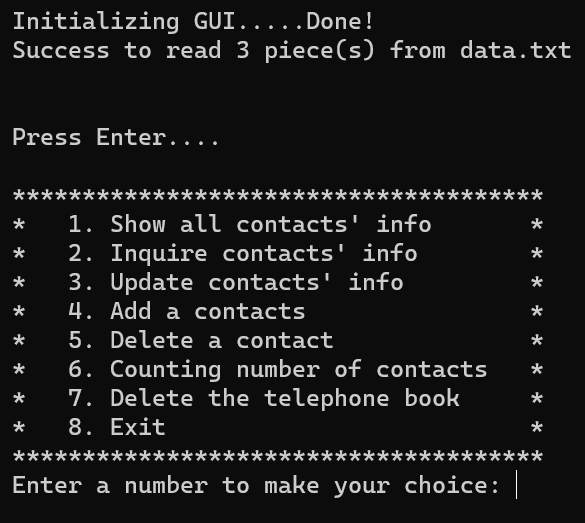
\includegraphics[width=0.3\textwidth]{graphic/01.png}
  \caption{初始化界面}
  \label{}
\end{figure}
初始化成功并显示成功读取数据。接下来测试读取数据是否正确。
\begin{figure}[!h]
  \centering
  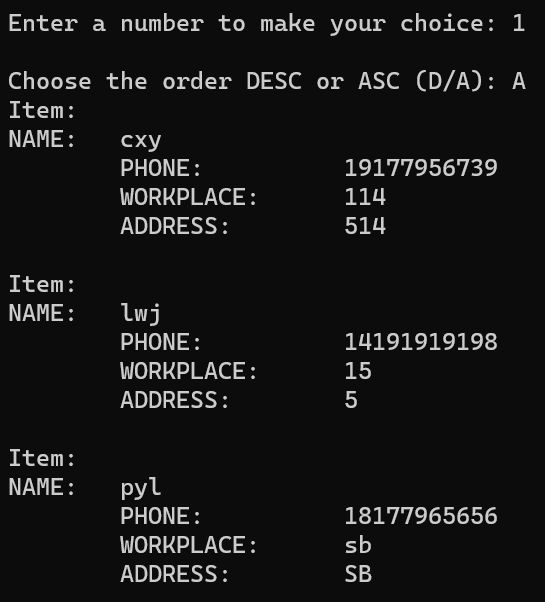
\includegraphics[width=0.3\textwidth]{graphic/02.png}
  \caption{采用字母升序(ASC)输出电话簿}
  \label{}
\end{figure}

本次操作结束,返回主界面测试查询功能。\newpage

\begin{figure}[!h]
  \centering
  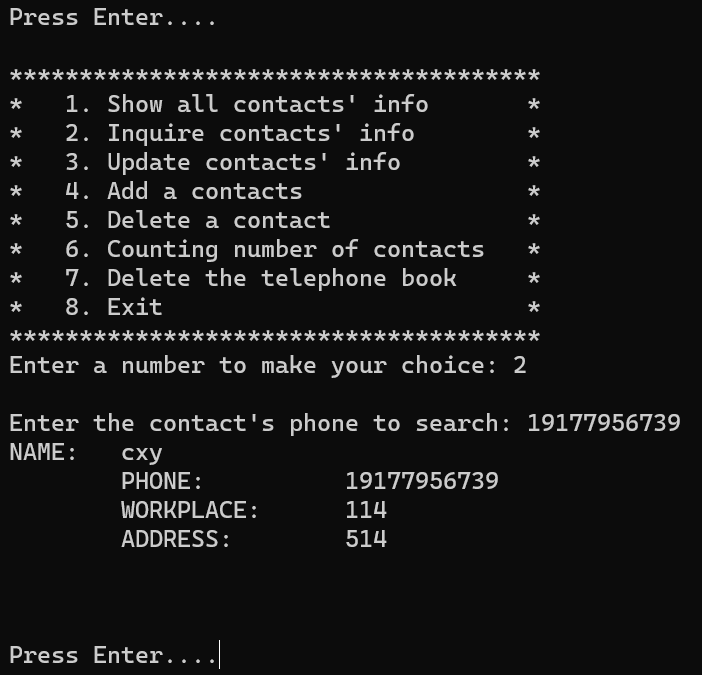
\includegraphics[width=0.3\textwidth]{graphic/03}
  \caption{成功根据电话查询联系人}
  \label{}
\end{figure}

测试修改联系人信息,按姓名检索:

\begin{figure}[!h]
\begin{minipage}{0.49\linewidth}
        \centering
        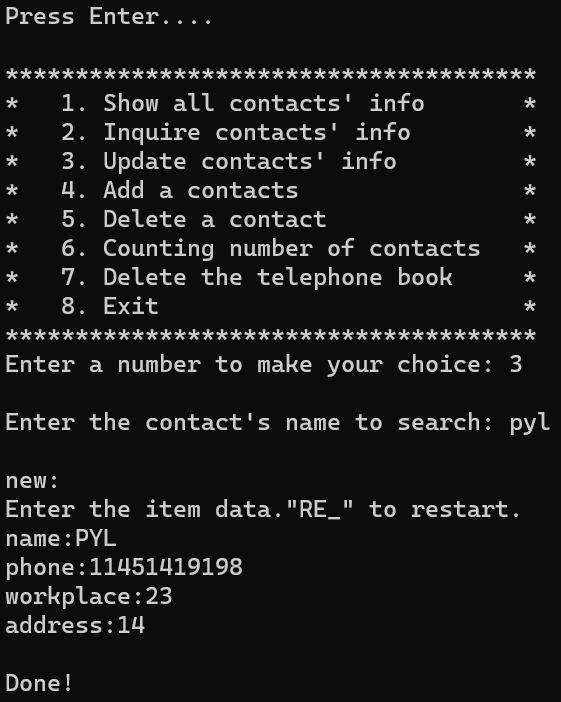
\includegraphics[width=0.6\textwidth]{graphic/04.png}
        \caption{执行修改联系人信息,提示成功}
        \label{}
\end{minipage}
%
\begin{minipage}{0.49\linewidth}
        \centering
        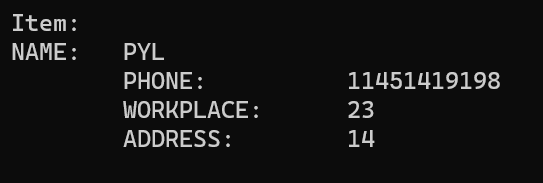
\includegraphics[width=0.9\textwidth]{graphic/05.png}
        \caption{更新后的联系人信息}
        \label{}
\end{minipage}
\end{figure}

测试插入联系人信息:可随时在字段中输入"RE\_{}"来重置添加;添加时会检查元素合法性,本例中只需要检查电话号码是否为11位纯数字。

\begin{figure}[!h]
    \begin{minipage}{0.49\linewidth}
            \centering
            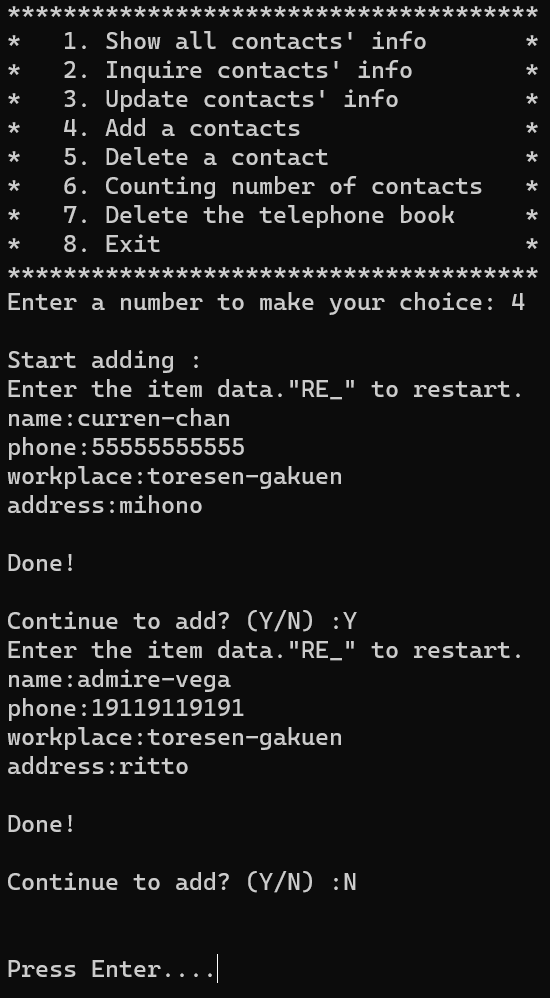
\includegraphics[width=0.5\textwidth]{graphic/06.png}
            \caption{成功连续添加}
            \label{}
    \end{minipage}
    %
    \begin{minipage}{0.49\linewidth}
            \centering
            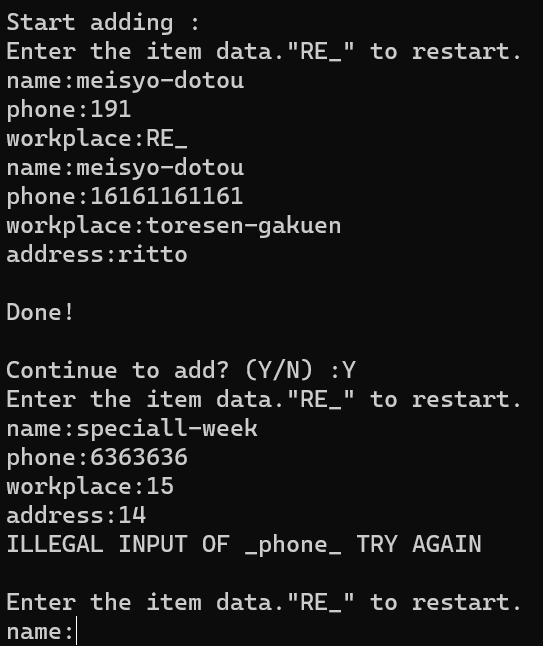
\includegraphics[width=0.7\textwidth]{graphic/07.png}
            \caption{两种错误情况}
            \label{}
    \end{minipage}
    \end{figure}

然后测试删除联系人操作:

\begin{figure}[!h]
    \begin{minipage}{0.49\linewidth}
            \centering
            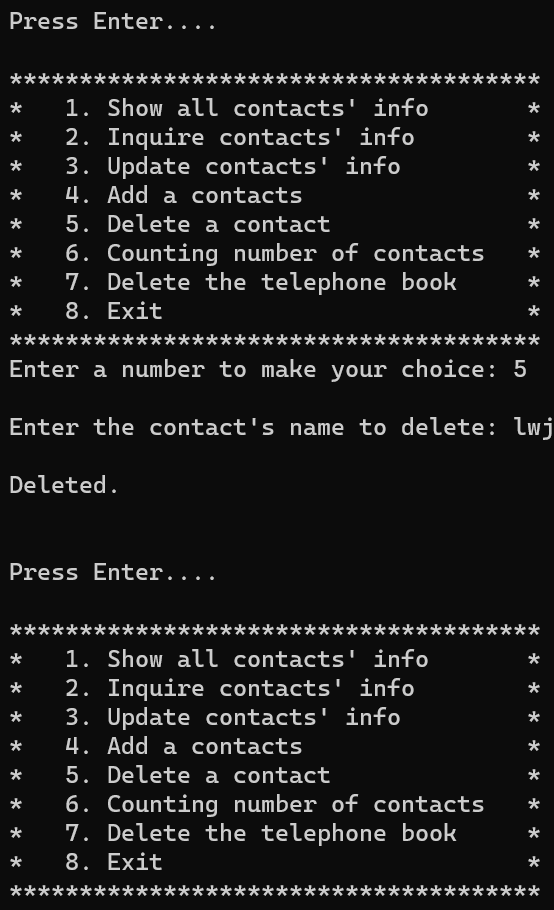
\includegraphics[width=0.65\textwidth]{graphic/08.png}
            \caption{显示成功删除“lwj”}
            \label{}
    \end{minipage}
    %
    \begin{minipage}{0.49\linewidth}
            \centering
            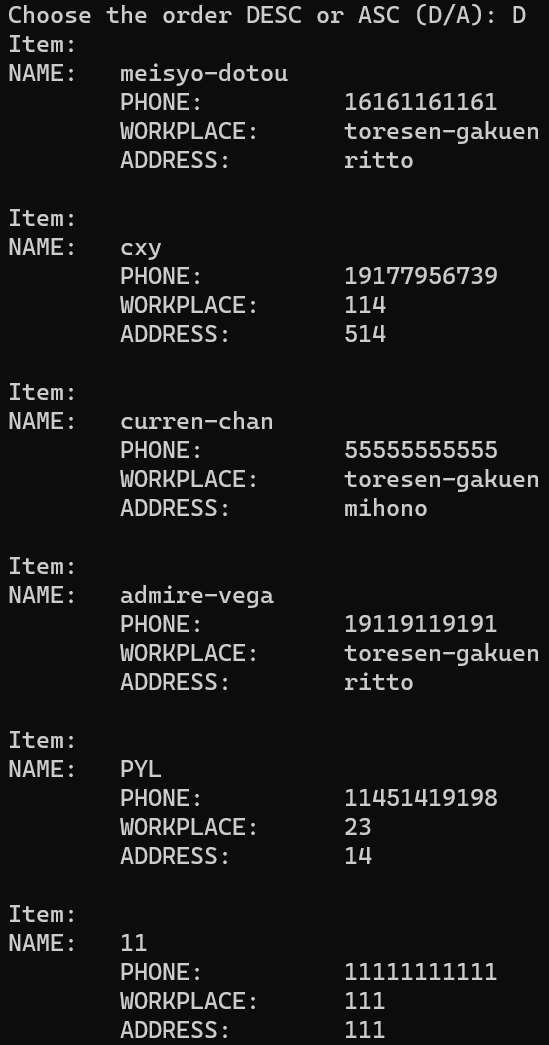
\includegraphics[width=0.6\textwidth]{graphic/09.png}
            \caption{删除后的元素列表}
            \label{}
    \end{minipage}
    \end{figure}

元素计数:
\begin{figure}[ht]
  \centering
  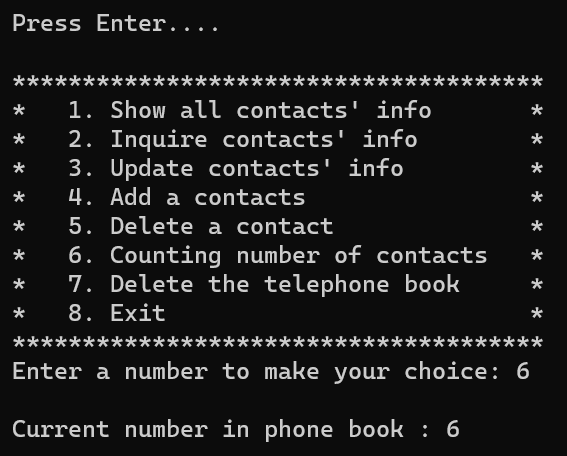
\includegraphics[width=0.4\textwidth]{graphic/10.png}
  \caption{正确显示当前树中有6个元素}
  \label{}
\end{figure}

选项7和选项8的区别在于:选项7会直接清空程序缓存中的树中的所有数据,然后回到主界面;而选项8会现将现有数据写入DATABASE指向的文件后退出程序,代码是;

\begin{framed}
\begin{lstlisting}[language=C++]
    ...
    case 7:
            fpw = fopen(DATABASE, "w");//清空文件
            DelAll(ptree);
            break;
        case 8:
            fpw = fopen(DATABASE, "w");
            TreeWritef(ptree, fpw, "ASC"); //默认升序写入
            DelAll(ptree);
            return 0;
            break;
    ...
\end{lstlisting}
\end{framed}

在这里只演示选项8,程序立即退出。打开data.txt文件

\begin{figure}[ht]
  \centering
  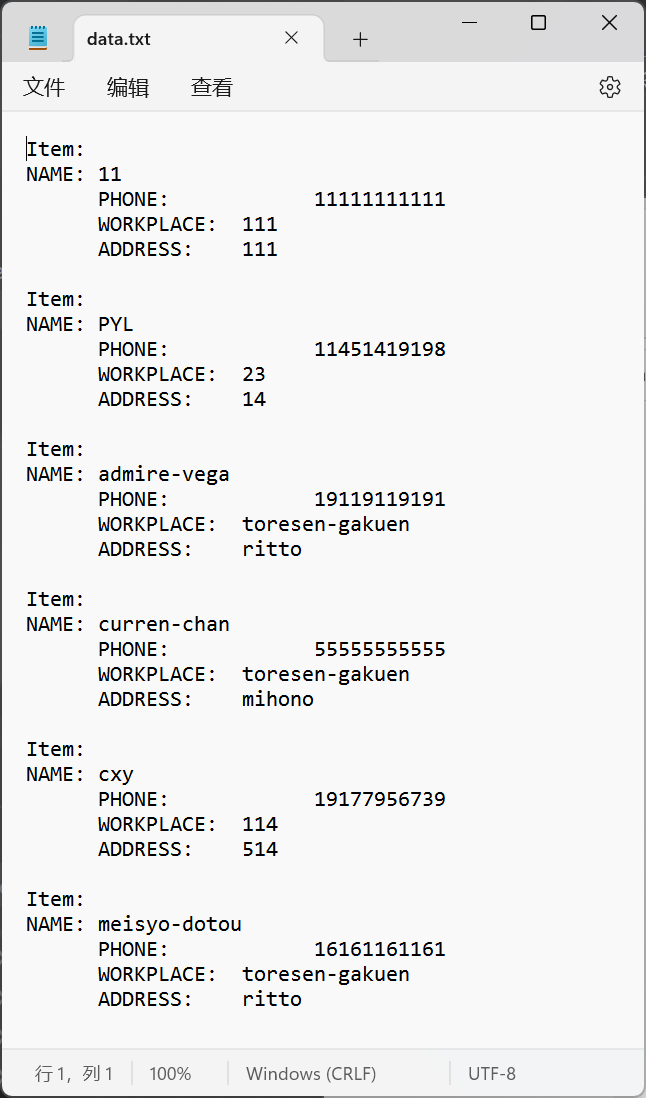
\includegraphics[width=0.35\textwidth]{graphic/11.png}
  \caption{数据被正确记录并写入文件}
  \label{}
\end{figure}

注意,必须执行选项8后才能将程序中操作的元素写入文件,否则文件的内容不会被修改。

\section{完整代码实现}

\begin{framed}
\begin{lstlisting}[language=C++]
    //AVLTree.h -AVL树ADT原型
    //树中不允许重复数据
    //左子树的所有项都在根节点的前面,右子树的所有项都在根节点的后面
    #pragma once
    #include <stdbool.h>
    #include <stdio.h>
    #include "Format.h"
    
    #ifndef MAXITEM
    #define MAXITEM (50) //树中最多元素个数
    #endif
    
    #ifndef DATABASE
    #define DATABASE "data.txt" //树中最多元素个数
    #endif
    
    /*定义结构*/
    
    //二叉树节点结构体
    typedef struct trnode
    {
        Item item;
        int height;
        struct trnode * left;
        struct trnode * right;
    } Trnode;
    
    //二叉树访问结构体
    typedef struct tree
    {
        Trnode * root;
        int size;
    } Tree;
    
    //二叉查找结构体
    typedef struct pair
    {
        Trnode * parent;
        Trnode * child;
    } Pair;
    
    /*函数原型*/
    
    //O:将树初始化为空
    //P:NULL
    //E:树被初始化为空,并返回一个指向Tree的指针
    Tree * InitializeTree(void);
    
    //O:确定树是否为空
    //P:ptree指向一个Tree类型
    //E:若为空,返回true,否则返回false
    bool IsTreeEmpty(const Tree * ptree);
    
    //O:确定树是否已满
    //P:ptree指向一个Tree类型
    //E:若为空,返回true,否则返回false
    bool IsTreeFull(const Tree * ptree);
    
    //O:确定树中的项数
    //P:ptree指向一个Tree类型
    //E:返回一个树的项数
    int TreeItemCount(const Tree * ptree);
    
    //O:在树中添加一个项
    //P:pi指向待添加项的地址,ptree指向要添加到的树
    //E:如果可以添加,则返回该节点及其父级
    bool AddItem(const Item * pi, Tree * ptree);
    
    //O:在树中删除一个项
    //P:pi指向待删除项的地址,ptree指向要操作的树
    //E:如果可以删除,则返回true,同时将该项从树中删除,否则返回false
    bool DelItem(const Item * pi, Tree * ptree);
    
    //O:在树中查找一个项
    //P:pi指向待查找项的地址,ptree指向要操作的树
    //E:如果查找到,则返回true,否则返回false
    bool InTree(const Item * pi, const Tree * ptree);
    
    //O:清空树
    //P:ptree指向一个Tree类型
    //E:ptree指向的Tree被清空
    void DelAll(Tree * ptree);
    
    //O:将通讯录写入指定文件流
    //P:ptree指向一个Tree类型,File指向一个文件
    //E:ptree指向的Tree中的每一个Item以指定顺序写入文件流
    bool TreeWritef(const Tree * ptree, FILE * fp, const char * order);
    
    //O:从指定文件流中读取一个树
    //P:ptree指向一个Tree类型,File指向一个文件
    //E:ptree指向的Tree中的每一个Item以指定顺序写入文件流并自平衡
    bool TreeReadf(Tree * ptree, FILE * fp);
    
    //O:在交互页面(标准输入流中)读取树的一个元素
    //P:ptree指向一个Tree类型
    //E:ptree指向的树中的Item写入文件流并自平衡
    bool TreeReadOne(Tree * ptree);
    
    //O:在输入流中显示二叉树结构
    //P:ptree指向一个Tree类型,fp是一个文件指针
    //E:ptree指向的树以图表方式显示在fp指向的文件流中,以name为标签
    bool ShowTree(Tree *ptree, FILE * fp);
    
    //O:在指定文件流中输出一个Item结构
    //P:fp是一个文件指针
    //E:在fp指向的文件中格式化打印了一个item中的数据
    bool PrintItem(const Item item, FILE * fp);
    
    //O:在树中搜索节点
    //P:pi指向一个Item结构,ptree指向一个Tree结构
    //O:值为pi指向的值的节点,返回以这个节点为子节点的Pair结构
    Pair SeekItem(const Item * pi, const Tree * ptree);
\end{lstlisting}
\end{framed}

\begin{framed}
\begin{lstlisting}[language=C++]
    //Format.h -电话簿信息结构定义
    #pragma once
    #define MAXLINE 20
    #define PHONENUMBERLINE 11 + 2
    //#define _DEBUG_MODE_ _DEBUG_MODE_ //debug模式开关-只使用name字段
    
    #ifndef _DEBUG_MODE_
    typedef struct item
    {
        char name[MAXLINE];
        char phone[PHONENUMBERLINE];
        char workplace[MAXLINE];
        char address[MAXLINE];
    } Item;
    
    #else
    typedef struct item
    {
        char name[MAXLINE];
    } Item;
    
    #endif
\end{lstlisting}
\end{framed}

\begin{framed}
\begin{lstlisting}[language=C++]
    //AVLTree.c -AVL树ADT基本代码
    #include <stdio.h>
    #include <string.h>
    #include <stdlib.h>
    #include <ctype.h>
    #include "AVLTree.h"
    #include "Format.h"
    
    //////////
    
    /*局部函数声明*/
    static bool ToLeft(const Item * i1, const Item * i2);
    static bool ToRight(const Item * i1, const Item * i2);
    static Pair RecuSeek(const Item * pi, Pair look);
    static Trnode * MakeNode(const Item * pi);
    static Trnode * AddNode(Trnode * new_node, Trnode * root);
    static Trnode * Rotation(Pair current);
    static int GetHeight(const Trnode * root);
    static int GetHeightFactor(const Trnode * root);
    static void ChangeHeight(Trnode * root, int val);
    static Trnode * RightRotate(Trnode * root);
    static Trnode * LeftRotate(Trnode * root);
    static void InOrder(const Trnode * parent, void(*pfun)(Item item));
    static void DelAllNodes(Trnode * root);
    static void DeleteNode(Trnode **ptr);
    static int Islegal(Item * pi);
    static bool PrintDESC(const Trnode * root, FILE * fp);
    static bool PrintASC(const Trnode * root, FILE * fp);
    #define MAX(a, b) (a) > (b) ? (a) : (b)
    /*函数代码*/
    
    Tree * InitializeTree(void)
    {
        Tree *ptree;
        ptree = (Tree *) malloc(1 * sizeof(Tree));
        ptree->root = NULL;
        ptree->size = 0;
        return ptree;
    }
    
    bool IsTreeEmpty(const Tree * ptree)
    {
        if(ptree->root == NULL)
            return true;
        else
            return false;
    }
    
    bool IsTreeFull(const Tree * ptree)
    {
        if(ptree->size >= MAXITEM)
            return true;
        else
            return false;
    }
    
    int TreeItemCount(const Tree * ptree)
    {
        return ptree->size;
    }
    
    bool InTree(const Item * pi, const Tree * ptree)
    {
        return (SeekItem(pi, ptree).child == NULL) ? false : true;
    }
    
    //节点导航
    static bool ToLeft(const Item * i1, const Item * i2)
    {
        int comp1;
        if((comp1 = strcmp(i1->name, i2->name)) < 0)
            return true;
        else
            return false;
    }
    
    static bool ToRight(const Item * i1, const Item * i2)
    {
        int comp1;
        if((comp1 = strcmp(i1->name, i2->name)) > 0)
            return true;
        else
            return false;
    }
    
    //搜索节点(递归方法)
    Pair SeekItem(const Item * pi, const Tree * ptree)
    {
        Pair look;
        look.parent = NULL;
        look.child = ptree->root;
        if(look.child == NULL)
            return look;
        else
            return RecuSeek(pi, look);
    }
    
    static Pair RecuSeek(const Item * pi, Pair look)
    {
        if(look.child == NULL)
            return look;
        else if(ToLeft(pi, &(look.child->item)))
        {
            look.parent = look.child;
            look.child = look.child->left;
            return RecuSeek(pi, look);
        }
        else if(ToRight(pi, &(look.child->item)))
        {
            look.parent = look.child;
            look.child = look.child->right;
            return RecuSeek(pi, look);
        }
        else 
            return look;
    }
    
    //插入节点
    bool AddItem(const Item * pi, Tree * ptree)
    {
        Trnode * new_node;
        if(IsTreeFull(ptree))
        {
            fprintf(stderr, "MEMORY FULL\n");
            return false;
        }
        if(SeekItem(pi, ptree).child != NULL)
        {
            fprintf(stderr, "DUPLICATE DATE\n");
            return false;
        }
        //用MakeNode函数创建节点并将new_node指向新节点
        new_node = MakeNode(pi);
        if(new_node == NULL)
        {
            fprintf(stderr, "CANNOT CRATE A NODE");
            return false;
        }
        if(ptree->root == NULL)
            ptree->root = new_node;
        else
            ptree->root = AddNode(new_node, ptree->root);
        ptree->size++;
        return true;
    }
    
    static Trnode * MakeNode(const Item * pi)
    {
        Trnode * new_node;
        new_node = (Trnode *) malloc(sizeof(Trnode));
        if(new_node != NULL)
        {
            new_node->item = *pi;
            new_node->left = NULL;
            new_node->right = NULL;
            new_node->height = 0; //节点高度初始化为0
        }
        return new_node;
    }
    
    static Trnode * AddNode(Trnode * new_node, Trnode * root)
    {   
        Pair current;
        current.parent = root;
        new_node->height = root->height + 1;  
        if(ToLeft(&new_node->item, &root->item))
        {  
            if(root->left == NULL)
            {
                root->left = new_node;
                current.child = root->left;
            }
            else
            {
                current.child = AddNode(new_node, root->left);//递归查找子树
                current.parent->left = current.child;
            }
        }
        else if(ToRight(&new_node->item, &root->item))
        {
            if(root->right == NULL)
            {
                root->right = new_node;
                current.child = root->right;
            }
            else
            {
                current.child = AddNode(new_node, root->right);//递归查找子树
                current.parent->right = current.child;
            }
        }
        else
        {
            fprintf(stderr, "FAIL TO ADD A NODE");
            exit(EXIT_FAILURE);
        }
        //添加完成后检测父节点高度因子,从下到上逐次旋转
        //高度因子为左最长子树高度-右,若为正数则R或LR,若为负数则L或RL
        return Rotation(current);
    }
    
    //执行旋转操作,返回新的根节点
    static Trnode * Rotation(Pair current)
    {
        int Rotate = GetHeightFactor(current.parent);
        if(Rotate > 1)
        {   
            if(GetHeightFactor(current.child) < 0)
                current.parent->left = LeftRotate(current.child);
            return RightRotate(current.parent);
        }
        else if(Rotate < -1)
        {   
            if(GetHeightFactor(current.child) > 0)
                current.parent->right = RightRotate(current.child);
            return LeftRotate(current.parent);
        }
        else
            return current.parent;
    }
    
    static int GetHeight(const Trnode * root)
    {   
        if(root == NULL)
            return 0;
        if(root->left == NULL && root->right == NULL)
            return root->height;
        else if(root->left == NULL && root->right != NULL)
            return GetHeight(root->right);
        else if(root->left != NULL && root->right == NULL)
            return GetHeight(root->left);
        else
            return MAX(GetHeight(root->left), GetHeight(root->right));
    }
    
    static int GetHeightFactor(const Trnode * root)
    {   
        if(root == NULL)
            return 0;
        else if(root->left == NULL && root->right != NULL)
            return root->height - GetHeight(root->right);
        else if(root->left != NULL && root->right == NULL)
            return GetHeight(root->left) - root->height;
        else
            return GetHeight(root->left) - GetHeight(root->right);
    }
    
    static void ChangeHeight(Trnode * root, int val)
    {
        if(root != NULL)
        {
            ChangeHeight(root->left, val);
            root->height += val;
            ChangeHeight(root->right, val);
        }
    }
    
    static Trnode * RightRotate(Trnode * root)
    {   
        Trnode * new_root = NULL;
        new_root = root->left;
        //左子树高度全部减1,右子树和根节点高度全部加1
        ChangeHeight(root->left, -1);
        root->height += 1;
        ChangeHeight(root->right, 1);
        //移动指针
        root->left = (new_root->right == NULL) ? NULL : new_root->right;
        new_root->right = root;
        return new_root;
    }
    
    static Trnode * LeftRotate(Trnode * root)
    {   
        Trnode * new_root = NULL;
        new_root = root->right;
        //右子树高度全部减1,左子树和根节点高度全部加1
        ChangeHeight(root->right, -1);
        root->height += 1;
        ChangeHeight(root->left, 1);
        //移动指针
        root->right = (new_root->left == NULL) ? NULL : new_root->left;
        new_root->left = root;
        return new_root;
    }
    
    //中序遍历-默认按首字母升序
    static void InOrder(const Trnode * parent, void(*pfun)(Item item))
    {
        if(parent != NULL)
        {
            InOrder(parent->left, pfun);
            (*pfun)(parent->item);
            InOrder(parent->right, pfun);
        }
    }
    
    //完全清空树
    void DelAll(Tree * ptree)
    {   
        if(ptree != NULL)
            DelAllNodes(ptree->root);
        else
            return;
        ptree->root = NULL;
        ptree->size = 0;
        free(ptree);
    }
    
    static void DelAllNodes(Trnode * root)
    {
        //中序遍历清空项
        Trnode * pright;
        if(root != NULL)
        {
            pright = root->right;
            DelAllNodes(root->left);
            free(root);
            DelAllNodes(pright);
        }
    }
    
    //删除某一元素
    bool DelItem(const Item * pi, Tree * ptree)
    {
        Pair look;
        look = SeekItem(pi, ptree);
        if(look.child == NULL)
            return false;
        if(look.parent == NULL)//根节点情形
            DeleteNode(&ptree->root);
        else if(look.parent->left == look.child)
            DeleteNode(&look.parent->left);
        else
            DeleteNode(&look.parent->right);
        ptree->size--;
        //检查是否平衡
        if(Rotation(look) != NULL)
            return true;
        else
            return false;
    }
    
    static void DeleteNode(Trnode **ptr)
    {
        Trnode * temp;
        if((*ptr)->left == NULL)
        {
            temp = *ptr;
            *ptr = (*ptr)->right;
            free(temp);
        }
        else if((*ptr)->right == NULL)
        {
            temp = *ptr;
            *ptr = (*ptr)->left;
            free(temp);
        }
        else
        //此时被删除的节点有两个子节点
        //在被删除节点的右支树中找到最近的空位并连上去
        {
            for(temp = (*ptr)->left; temp->right != NULL; temp = temp ->right)
                continue;
            temp->right = (*ptr)->right;
            temp = *ptr;
            *ptr = (*ptr)->left;
            free(temp);
        }
    }
    
    bool TreeWritef(const Tree * ptree, FILE * fp, const char * order)
    {
        if(ptree == NULL)
        {
            return false;
            fprintf(stderr, "TREE DOES NOT EXISTS");
        }
        if(strcmp(order, "DESC"))
            return PrintDESC(ptree->root, fp);
        if(strcmp(order, "ASC"))
            return PrintASC(ptree->root, fp);
        return false;
    }
    
    static bool PrintASC(const Trnode * root, FILE * fp)
    {   
        if(root != NULL)
        {
            PrintASC(root->right, fp);
            fprintf(fp, "Item:\n");
            PrintItem(root->item, fp);
            PrintASC(root->left, fp);
        }
    }
    
    static bool PrintDESC(const Trnode * root, FILE * fp)
    {   
        if(root != NULL)
        {
            PrintDESC(root->left, fp);
            fprintf(fp, "Item:\n");
            PrintItem(root->item, fp);
            PrintDESC(root->right, fp);
        }
    }
    
    bool PrintItem(const Item item, FILE * fp)
    {
        fprintf(fp, "NAME:\t%s\n", item.name);
        fprintf(fp, "\tPHONE:\t\t%s\n", item.phone);
        fprintf(fp, "\tWORKPLACE:\t%s\n", item.workplace);
        fprintf(fp, "\tADDRESS:\t%s\n\n", item.address);
    
        return true;
    }
    
    bool TreeReadf(Tree * ptree, FILE * fp) 
    {
        char line[MAXLINE + 50] = {'\0'};//这里挺容易溢出的
        Item item;
        int count = 0;
        while (fgets(line, sizeof(line), fp) != NULL) 
        {   // 逐行读取文件内容
            int i = 0;
            while(line[i] == ' ' || line[i] == '\n' || line[i] == '\t')
                    ++i;//跳过空白符
            if (line[i] == 'N' && line[i + 1] != 'o')
                sscanf(line + i, "NAME: %s", item.name); 
            else if (line[i] == 'P') 
                sscanf(line + i, "PHONE: %s", item.phone); 
            else if (line[i] == 'W')
                sscanf(line + i, "WORKPLACE: %s", item.workplace);
            else if (line[i] == 'A')
            {
                sscanf(line + i, " ADDRESS: %s", item.address); 
                if(!AddItem(&item, ptree))
                    return false;
                ++count;
            }
            else
                continue;
        }
        fprintf(stdout, "Success to read %d piece(s) from "DATABASE"\n", count);
        return true;
    }
    
    bool TreeReadOne(Tree * ptree)
    {
        if(ptree == NULL)
        {
            return false;
            fprintf(stderr, "TREE DOES NOT EXISTS");
        }
        Item * pi = (Item *) malloc(sizeof(Item));
        fputs("Enter the item data.\"RE_\" to restart.\n", stdout);
        const char *filed[] = {"EMPTY", "name", "phone", "workplace", "address"};
        int i = 1;
        for(i = 1; i <= 4; ++i)
        {
            fprintf(stdout, "%s:", *(filed+i));        
            char temp[MAXLINE] = {'\0'};
            fscanf(stdin, "%s", temp);
            if(strcmp(temp, "RE_") == 0)
            {
                i = 0;
                continue;
            }
            if(i == 1)
                strcpy(pi->name, temp);
            if(i == 2)
                strcpy(pi->phone, temp);
            if(i == 3)
                strcpy(pi->workplace, temp);
            if(i == 4)
                strcpy(pi->address, temp);
        }
        int wrong = Islegal(pi);
        if(wrong > 0)
        {
            fprintf(stdout, "ILLEGAL INPUT OF _%s_ TRY AGAIN\n\n", filed[wrong]);
            TreeReadOne(ptree);
        }
        else if(!AddItem(pi, ptree))
        {
            fprintf(stderr, "FAIL TO INSERT\n");
            free(pi);
            return false;
        }
        free(pi);
        fprintf(stdout,"\nDone!\n");
        return true;
    }
    
    //检测输入是否合法,若有错误则返回错误项标号,否则返回0
    static int Islegal(Item * pi)
    {
        if(strlen(pi->phone) != 11)
            return 2;
        for(int i = 0; i < 11; ++i)
            if((pi->phone)[i] < '0' || (pi->phone)[i] > '9')
                return 2;
        return 0;
        //目前只要求检测电话号码的合法性
    }
\end{lstlisting}
\end{framed}

\begin{framed}
\begin{lstlisting}[language=C++]
    //TelephoneBook.c -程序主函数&图形化界面
    #include <stdio.h>
    #include <stdlib.h>
    #include <ctype.h>
    #include <string.h>
    #include <stdbool.h>
    #include "AVLTree.h"
    #include "Format.h"
    //#define DATABASE diyname
    //局部函数声明
    static int ShowGUI(void);
    static bool ShowAllContacts(Tree * ptree);
    static bool UpdateContact(Tree * ptree, char *phone);
    static int IsContact(const Trnode * root, char *name, FILE * fp);

    int main(void)//日后可加启动参数
    {
        printf("Initializing GUI.....Done!\n");
    
        FILE * fpr = fopen(DATABASE, "r");
        FILE * fpw = NULL;
        Tree * ptree = InitializeTree();
        char line[MAXLINE] = {'\0'};
        if(!TreeReadf(ptree, fpr))
        {
            fprintf(stderr, "FAIL TO READ FROM FILE\n");
            exit(EXIT_FAILURE);
        }
        int choice = 7;
        while(true)
        {   
            printf("\n\nPress Enter....");
            getchar();
            choice = ShowGUI();
            if(choice == 0)
            {
                fprintf(stderr, "FAIL TO SHOW GUI\n");
                exit(EXIT_FAILURE);
            }
            switch (choice)
            {
            case 1:
                if(!ShowAllContacts(ptree))
                    printf("FAIL TO SHOW ALL CONTACTS");
                break;
            case 2:
                printf("\nEnter the contact's phone to search: ");
                scanf("%s", line);getchar();
                if(IsContact(ptree->root, line, stdout) == 0)
                    printf("\nNo data found.\n");
                break;
            case 3:
                printf("\nEnter the contact's name to search: ");
                scanf("%s", line);getchar();
                UpdateContact(ptree, line);
                break;
            case 4:
                printf("\nStart adding :\n");
                char ch = 'Y';
                while(true)
                {
                    TreeReadOne(ptree);
                    printf("\nContinue to add? (Y/N) :");
                    getchar();scanf("%c", &ch);getchar();
                    if(ch == 'Y')
                        continue;
                    else
                        break;
                }
                break;
            case 5:
                printf("\nEnter the contact's name to delete: ");
                scanf("%s", line);getchar();
                Item item;
                strcpy(item.name, line);
                Trnode *node;
                node = SeekItem(&item, ptree).child;
                if(node == NULL)
                {
                    printf("\nFind no data.\n");
                    break;
                }
                else
                    DelItem(&(node->item), ptree);
                printf("\nDeleted.\n");
                break;
            case 6:
                printf("\nCurrent number in phone book : %d \n", TreeItemCount(ptree));
                break;
            case 7:
                fpw = fopen(DATABASE, "w");//清空文件
                DelAll(ptree);
                break;
            case 8:
                fpw = fopen(DATABASE, "w");
                TreeWritef(ptree, fpw, "ASC"); //默认升序写入
                DelAll(ptree);
                return 0;
                break;
            case 114514:
                ShowTree(ptree, stdout);
                getchar();
                break;
            default:
                printf("Wrong choice!Try again.\n");
                break;
            }
        }
        return 0;
    }
    static int ShowGUI(void)
    {
        printf("\n**************************************\n");
        printf("*   1. Show all contacts' info       *\n");
        printf("*   2. Inquire contacts' info        *\n");
        printf("*   3. Update contacts' info         *\n");
        printf("*   4. Add a contacts                *\n");
        printf("*   5. Delete a contact              *\n");
        printf("*   6. Counting number of contacts   *\n");
        printf("*   7. Delete the telephone book     *\n");
        printf("*   8. Exit                          *\n");
        printf("**************************************\n");
        printf("Enter a number to make your choice: ");
    
        int n;
        scanf("%d", &n);
        return n;
    }
    static bool ShowAllContacts(Tree * ptree)
    {
        char order = 0;
        while(true)
        {
            printf("\nChoose the order DESC or ASC (D/A): ");
            getchar();scanf("%c", &order);getchar();
            if(order == 'D')
            {
                TreeWritef(ptree, stdout, "DESC");
                return true;
            }
            else if(order == 'A')
            {
                TreeWritef(ptree, stdout, "ASC");
                return true;
            }
            printf("WRONG ORDER (A/D)\n");
        }
        return false;
    }
    
    static int IsContact(const Trnode * root, char *phone, FILE * fp)
    {   
        static int count = -1;
        if(root != NULL)
        {
            IsContact(root->left, phone, fp);
            if(!strcmp((root->item.phone), phone))
                PrintItem(root->item, fp);
            IsContact(root->right, phone, fp);
        }
        ++count;
        return count;
    }
    
    static bool UpdateContact(Tree * ptree, char *name)
    {   
        Item item;
        strcpy(item.name, name);
        Trnode *node = SeekItem(&item, ptree).child;
        if(node == NULL)
        {
            printf("\nFind no data. Add a contact?");
            return false;
        }
        else
        {
            DelItem(&(node->item), ptree);
            printf("\nnew: \n");
            TreeReadOne(ptree);
        }
        return true;
    }
\end{lstlisting}
\end{framed}

\section{总结}
通过这次大作业,我进一步掌握了C语言程序设计的基本语法、方法,能够做到熟练运用指针进行面向过程的编程,掌握了二叉树数据结构的处理和实现,并尝试利用抽象数据类型(ADT)来实现接口和封装,从而编写一个较为复杂的程序。

但在过程当中,也存在一些问题,例如接口中各函数通信效率低,有时不得不复用一大段代码,造成结构不够明确、语法不够简洁、代码可读性差。这或许也是C语言的一个弱点,就是难以很好地进行模块化设计——或者说“面向对象编程”。以后我会尝试用C++将这些代码更细致、更有条理地封装在“类”之中。

同时我也发现对于一些比较复杂的数据结构,自己编写接口实现是比较困难的。这时就可以利用他人已经写好的代码,也就是“库”来帮助编程。这时库中的函数和方法对我们来说就是完全黑箱的“抽象数据类型”,我们只需调用即可。

\section*{编辑环境}
    代码编辑:Microsoft Visual Studio Code

    编译器:gcc 6.4.0 
    
    文档编辑:\LaTeX 2

\end{document}